\documentclass[aspectratio=169]{beamer}
\usetheme{metropolis}
\setbeamercovered{transparent} % Rende i punti successivi trasparenti finché non clicchi
\usepackage{tabularx}
\usepackage{graphicx}
\usepackage{booktabs}
\graphicspath{{img/}} % Cerca le immagini nella cartella img/
% \usepackage[style=numeric, sorting=none, backend=biber]{biblatex}
%\addbibresource{references.bib} % Il nome del file creato sopra

% ============================================================================
%  STRUCTURE SKELETON — rebuilt 2026-06-18
%  Legend used throughout this file:
%    % [KEEP]        slide content is current, no change needed
%    % [UPDATED]     numbers/text refreshed from results on disk (2026-06-18)
%    % [TODO]        placeholder — insert your own text / figure / numbers
%  Search this file for "TODO" to find everything still to fill in.
%
%  Section map:
%    1. Introduction            (IBD biology)                       [KEEP]
%    2. Project overview        (full-pipeline roadmap, goals)      [KEEP]
%    3. Phase 1 — Data & GenNet (dataset, PLINK, prep, mapping)     [KEEP]
%    4. Phase 2 — Methodological comparison
%         grid search + activation choice                          [UPDATED]
%         multi-seed stability (AUC + importance ranking)          [TODO/partial]
%    5. Phase 3 — Gene importance & ISN construction               [TODO/partial]
%    6. Phase 4 — HotZone analysis & proof of concept              [TODO]
%    7. Conclusions
%    8. References + closing                                       [KEEP]
% ============================================================================

% --- RIMUOVI LE ICONE (Libri/Documenti) ---
\setbeamertemplate{bibliography item}{\insertbiblabel}

% Riduce il font per la bibliografia (standard nelle presentazioni)
%\renewcommand*{\bibfont}{\scriptsize}

\title{MSc Thesis}
\subtitle{\small Integrating GenNet and ISNs for IBD Analysis}
\author{
  Kristian Kovacev\inst{1} \\
  \vspace{0.3cm}
  {\small Supervisors:} \\
  {\small Prof. Fabio Stella\inst{1} \quad Prof. Kristel Van Steen\inst{2}}
}

\date{June 18, 2026}

\institute{
    \inst{1} Università degli Studi di Milano-Bicocca \\
    \inst{2} Université de Liège (ULiège)
}

\begin{document}

\maketitle

% ============================================================================
\section{Introduction}
% ============================================================================

\begin{frame}{Biological Context: Inflammatory Bowel Disease (IBD)}
    % [KEEP]
    \begin{columns}[T]
        \begin{column}{0.55\textwidth}
            \begin{itemize}
                \item<1-> We investigated the \textbf{IBD dataset} from the International Inflammatory Bowel Disease Genetics Consortium (\textbf{IIBDGC}).
                \vspace{0.4cm}
                \item<2-> The data contains cases with \textbf{non-infectious inflammations} of the bowel, including:
                \begin{itemize}
                    \item \textbf{Ulcerative Colitis (UC)}
                    \item \textbf{Crohn’s Disease (CD)}
                \end{itemize}\label{key}

               \vspace{0.4cm}
                \item<3-> These represent the two main categories of IBD \cite{Strober2007}, characterized by distinct patterns of intestinal involvement.
            \end{itemize}
        \end{column}

        \begin{column}{0.45\textwidth}
            \centering
            \begin{figure}
                \includegraphics[width=\textwidth]{img/CGH-Patient-Ed-IBD2.0-2019.jpg}
                \caption{\small Comparison of UC and CD pathology.}
            \end{figure}
        \end{column}
    \end{columns}

\end{frame}

% ============================================================================
\section{Project overview}
% ============================================================================

\begin{frame}{Project Timeline: A 4-Month Roadmap}
    % [KEEP] — roadmap matches docs/project_context.md §2
    \begin{itemize}
        \item<1-> \textbf{Phase 1: Reproduce and Adapt}
            \begin{itemize}
                \item Setup GenNet pipeline and preparing input data.
            \end{itemize}
        \vspace{0.3cm}
        \item<2-> \textbf{Phase 2: Methodological Comparison}
            \begin{itemize}
                \item Testing activation functions and hyperparameters.
                \item Focus on \textbf{stability} of gene rankings and importance measures.
            \end{itemize}
        \vspace{0.3cm}
        \item<3-> \textbf{Phase 3: ISN Construction Strategy}
            \begin{itemize}
                \item Linking GenNet outputs to \textbf{Individual-Specific Networks} (ISNs).
                \item Testing node/edge definitions for HotZone-related signals.
            \end{itemize}
        \vspace{0.3cm}
        \item<4-> \textbf{Phase 4: HotZone Analysis}
            \begin{itemize}
                \item Detecting \textbf{HotZones} from the per-patient ISNs (high-variance edge communities).
                \item Scoring their \textbf{``hotness''}: differential wiring (D) and pathway enrichment (E).
            \end{itemize}
    \end{itemize}
\end{frame}

\begin{frame}{Goals and Expected Impact}
    % [KEEP]
    \begin{block}{Scientific Value}
        \begin{itemize}
            \item Demonstrate the promise of \textbf{post-GWAS analyses} linked to GenNet for the IIBDGC.
        \end{itemize}
    \end{block}

    \begin{block}{Practical Application}
        \begin{itemize}
            \item Development of a robust pipeline for \textbf{HotZone-aware} analysis.
            \item Integration of genomic data (SNPs) with high-level biological interactions.
        \end{itemize}
    \end{block}
\end{frame}

% ----------------------------------------------------------------------------
% OPTIONAL NEW SLIDE [TODO]: end-to-end pipeline diagram
% The supervisor's clarification (project_context.md §2) stresses evaluating the
% WHOLE pipeline per configuration: train -> gene importance -> ISN -> HotZone.
% A single overview figure here sets up Phases 2-4 as one continuous flow.
% ----------------------------------------------------------------------------
\begin{frame}{The End-to-End Pipeline}
    % [TODO] insert pipeline figure: SNP -> GenNet -> importance -> ISN -> HotZone
    \begin{figure}
        \centering
        % \includegraphics[width=0.9\linewidth]{img/pipeline_overview.png}
        \fbox{\parbox[c][4cm][c]{0.9\linewidth}{\centering
            \textit{[TODO: full-pipeline diagram]}\\[0.3cm]
            GenNet (train) $\rightarrow$ gene/pathway importance $\rightarrow$
            reference network $\rightarrow$ ISN per patient $\rightarrow$ HotZone scoring}}
        \caption{Each configuration is carried end-to-end and judged on the final HotZone objective.}
    \end{figure}
\end{frame}

% ============================================================================
\section{Phase 1 — Data \& GenNet setup}
% ============================================================================

\begin{frame}{Dataset Overview}
    % [KEEP]
    \begin{columns}[T]
        \begin{column}{0.45\textwidth}
        Van Hilten at al. \cite{vanHilten2025} performed \textbf{quality control} as in Ellinghaus et al. \cite{Ellinghaus2016}, reducing the number of SNPs from 196,524 to 130,071.
        \pause


        The final dataset contained \textbf{66,280 samples}, including \textbf{32,622 cases} (individuals with IBD) and \textbf{33,658 controls}.
        \pause
        The same quality control steps as in Duroux et al. \cite{duroux2022interpretable} were applied. They
        removed rare variants (MAF $<$ 5\%) or in Hardy-Weinberg equilibrium
        (p-value $<$ 0.001). All risk SNPs described in Liu et al. \cite{liu2015association} were included.
        \end{column}

        \begin{column}{0.55\textwidth}
                \centering
                \begin{figure}
                    \includegraphics[width=\textwidth]{img/IBD_QC.png}
                    \caption{\small IBD dataset after quality control.}
                \end{figure}
        \end{column}
    \end{columns}

\end{frame}

\begin{frame}{GenNet overview}
	 \begin{figure}
		\centering
		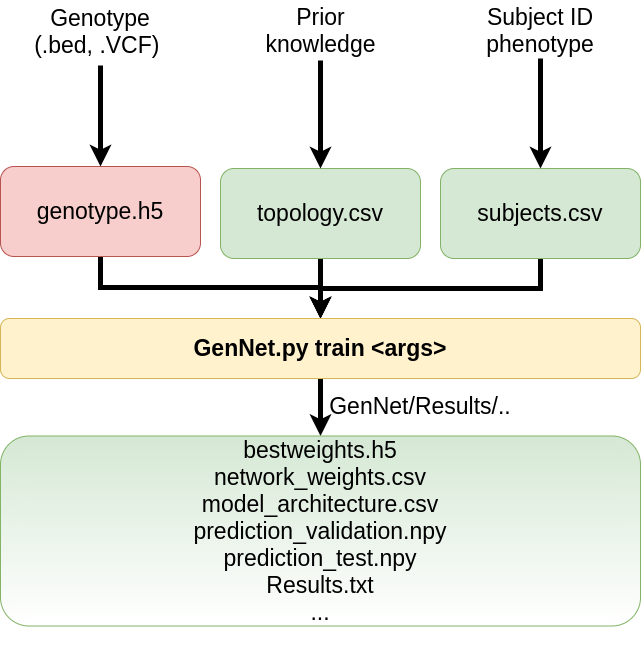
\includegraphics[width=0.45\linewidth]{img/Gennet_wiki_overview.png}
		\caption{\small From genotype to the masked network.}
	\end{figure}
\end{frame}

\begin{frame}{PLINK File}
    % [KEEP]
    \begin{itemize}
        \item \textbf{.bed}: \textbf{Binary Genotype File}. Stores genotypes (0/0, 0/1, 1/1, missing) using 2-bit compressed encoding for computational efficiency.
        \vspace{0.5cm}
        \item \textbf{.bim}: \textbf{Extended Variant Information}. Maps variant IDs to genomic positions and specific alleles.

        \vspace{0.5cm}
        \item \textbf{.fam}: \textbf{Sample Information}. Links samples to pedigree, sex, and clinical phenotype (case/control status).

    \end{itemize}
\end{frame}

\begin{frame}{First Step: GenNet Setup \& Data Conversion}
    % [KEEP]
    \small
    \textbf{Objective:} Convert PLINK files to GenNet formats for training.

    \vspace{0.4cm}

    \begin{columns}[T]
        \begin{column}{0.48\textwidth}
            \metroset{block=fill}
            \begin{block}{Input Data}
                \textbf{\texttt{genotype.h5}} \\
                Matrix: Samples $\times$ Variants.

                \vspace{0.3cm}

                \textbf{\texttt{subjects.csv}} \\
                Metadata \& Data Splits:
                \begin{itemize}
                    \item \texttt{labels}: Case/Control (0/1).
                    \item \texttt{genotype\_row}: Matrix index.
                    \item \texttt{set}: Train/Val/Test split.
                    \item \texttt{cov}: 7 PCs \cite{Ellinghaus2016}
                \end{itemize}
            \end{block}
        \end{column}

        \begin{column}{0.48\textwidth}
            \metroset{block=fill}
            \begin{block}{Network Structure}
                \textbf{\texttt{topology.csv}} \\
                The core of the NN design:
                \begin{itemize}
                    \item Maps paths from SNPs $\rightarrow$ Genes $\rightarrow$ Outcome.
                    \item Encodes \textbf{biological prior knowledge}.
                \end{itemize}
            \end{block}
        \end{column}
    \end{columns}
\end{frame}

\begin{frame}{Data Splitting Strategy}
    % [KEEP] — 65/20/15 stratified split, per-seed (docs/pipeline.md Step 3a)
   \begin{flushleft}
        I used the same splitting strategy as Van Hilten et al. \cite{vanHilten2025}.
    \end{flushleft}
    \vspace{0.8cm}
    {
    \centering


    \begin{columns}[onlytextwidth, c]
        \begin{column}{0.33\textwidth}
            \centering
            {\fontsize{45}{60}\selectfont \textbf{65\%}} \\
            \vspace{0.4cm}
            \huge \textsc{Train}
        \end{column}

        \begin{column}{0.33\textwidth}
            \centering
            {\fontsize{45}{60}\selectfont \textbf{20\%}} \\
            \vspace{0.4cm}
            \huge \textsc{Validation}
        \end{column}

        \begin{column}{0.33\textwidth}
            \centering
            {\fontsize{45}{60}\selectfont \textbf{15\%}} \\
            \vspace{0.4cm}
            \huge \textsc{Test}
        \end{column}
    \end{columns}
    \par
    }
    \vfill
    \vspace{0.5cm}
\end{frame}

\begin{frame}{Data Splitting}
    % [KEEP]
    \begin{figure}
        \centering
        \includegraphics[width=0.55\linewidth]{img/splitting.png}
        \caption{Final dataset after QC and data splitting}
    \end{figure}
\end{frame}

\begin{frame}{Functional Mapping with Annovar (hg19)}
    % [KEEP] — note Step 2d/2e (intergenic two-gene fix) is in pipeline.md if you
    % want to add a slide on the topology fixes you implemented.
    \textbf{Objective:} Map 38,225 SNPs to genomic coordinates and host genes.

    \begin{columns}[T]
        \begin{column}{0.50\textwidth}
            \metroset{block=fill}
            \begin{block}{Variant Categorization}
                \small
                \begin{itemize}
                    \item \textbf{Intragenic:} SNP inside a gene.
                    \item \textbf{Intergenic:} SNP between genes.
                    \item Mapped to \textbf{two nearest genes} with base-pair distance weight ($dist$).
                \end{itemize}
            \end{block}
        \end{column}
        \pause
        \begin{column}{0.45\textwidth}
            \metroset{block=fill}
            \begin{block}{The Goal}
                \small
                Transforms raw coordinates into a \textbf{functional map} for GenNet.
            \end{block}
        \end{column}
    \end{columns}

    \vspace{0.3cm}
    \pause
    \begin{block}{Data Transformation: "Exploding" the Mapping}
        \small
        \textbf{Problem:} The model cannot parse complex strings (e.g., \texttt{"Gene1, Gene2"}). \\
        \textbf{Solution:} Explode entries into independent observations for statistical aggregation.

        \vspace{0.2cm}
        \centering
        \begin{tabular}{l c l}
            \texttt{SNP\_A $\rightarrow$ "Gene1(X), Gene2(Y)"} & \textbf{$\Longrightarrow$} &
            \begin{tabular}{l} \texttt{SNP\_A $\rightarrow$ Gene1} \\ \texttt{SNP\_A $\rightarrow$ Gene2} \end{tabular}
        \end{tabular}
    \end{block}
\end{frame}

% ----------------------------------------------------------------------------
% NEW SLIDE [UPDATED 2026-06-18]: the CPDB pathway layer + pruning of genes
% without any pathway. Numbers verified from the topology files on disk:
%   pre-CPDB  (processed_data/old/topology_nopath.csv): 55,551 rows | 11,557 genes | 38,211 SNPs
%   final     (processed_data/topology.csv)           : 567,574 rows | 6,072 genes | 4,513 pathways | 25,576 SNPs
% ----------------------------------------------------------------------------
\begin{frame}{Adding the Pathway Layer: ConsensusPathDB (CPDB)}
    \small
    \begin{block}{Gene $\rightarrow$ Pathway mapping}
        \begin{itemize}
            \item Each gene (\texttt{layer1}) is joined to its \textbf{CPDB} pathways, forming the second hidden layer (\texttt{layer2}).
            \item CPDB chosen over Enrichr: it leaves \textbf{fewer genes without any pathway}.
            \item A gene belongs to \textbf{many} pathways $\rightarrow$ the merge \emph{expands} the table to one row per SNP--gene--pathway path.
        \end{itemize}
    \end{block}

    \begin{block}{Pruning genes without a pathway}
        \small
        After the merge, genes with \textbf{no CPDB pathway} have no \texttt{layer2} connection
        (\texttt{layer2\_node}~$=-1$). These rows are \textbf{removed} $\rightarrow$ genes drop from
        \textbf{11{,}557} to \textbf{6{,}072}.
    \end{block}

    \centering
    \scriptsize
    \renewcommand{\arraystretch}{1.2}
    \begin{tabular}{l c c}
        \toprule
        & \textbf{After Annovar} & \textbf{After CPDB + pruning} \\
        & (SNP\,$\rightarrow$\,gene) & (SNP\,$\rightarrow$\,gene\,$\rightarrow$\,pathway) \\
        \midrule
        Rows            & 55{,}551 & 567{,}574 \\
        Unique genes    & 11{,}557 & \textbf{6{,}072} \\
        Connected SNPs  & 38{,}211 & 25{,}576 \\
        Unique pathways & --       & 4{,}513 \\
        \bottomrule
    \end{tabular}
\end{frame}


\begin{frame}{GenNet framework}
	\begin{figure}
		\centering
		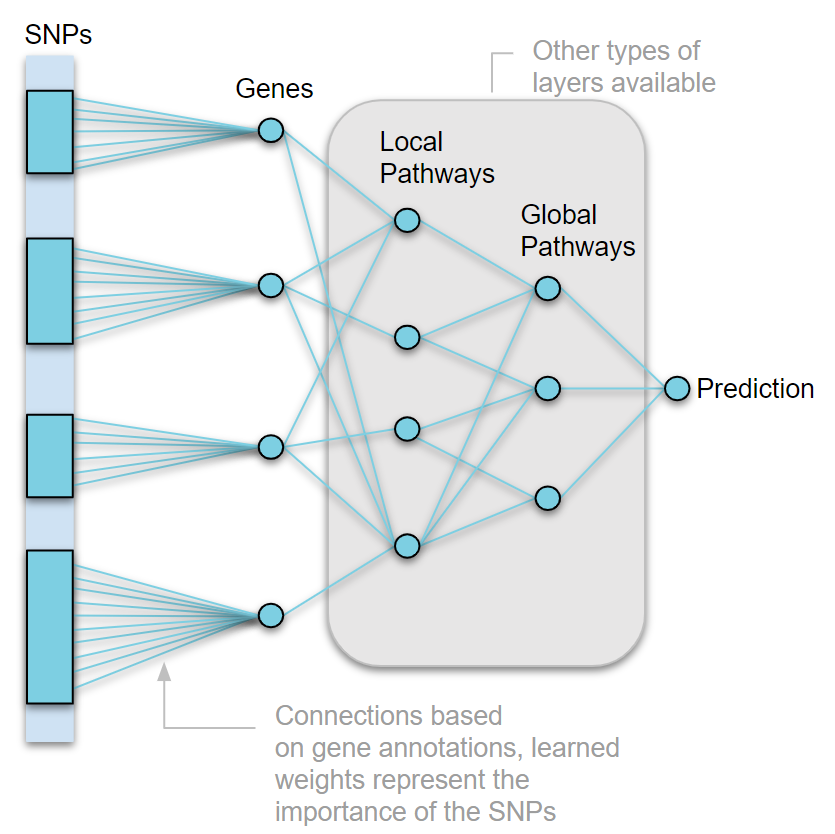
\includegraphics[width=0.45\linewidth]{img/figure1_github.PNG}
		\caption{\small Overview of the GenNet framework.}
	\end{figure}
\end{frame}

\begin{frame}{GenNet: Interpretable Deep Learning for Genetics}
    % [KEEP]
    \textbf{What is GenNet?} \\
    GenNet \cite{hilten2021gennet} is a framework for predicting phenotype from genotype. In this framework, prior knowledge is used to create groups of connected
nodes to reduce the number of learnable parameters in comparison to a fully connected neural network.

    \vspace{0.4cm}

    \begin{columns}[T]
        \begin{column}{0.6\textwidth}
            \metroset{block=fill}
            \begin{block}{Interpretable Connections}
                \small
                Instead of fully-connected layers, GenNet uses \textbf{biologically defined masks}:
                \begin{itemize}
                    \item \textbf{Layer 1:} SNPs $\rightarrow$ Genes (via annotations).
                    \item \textbf{Layer 2:} Genes $\rightarrow$ Pathways/Complexes.
                    \item \textbf{Layer 3:} Pathways $\rightarrow$ Phenotype.
                \end{itemize}
            \end{block}

        \end{column}
        \pause
            \begin{column}{0.48\textwidth}
            \metroset{block=fill}
            \begin{block}{Interpretation Module}
                \footnotesize
                GenNet extracts importance using:
                \begin{itemize}
                    \item \textbf{Weight Scores:} Global importance of features.
                    \item \textbf{Gradient-based attribution (SHAP):} per-feature importance.
                    \item \textbf{Interactions:} methods to find epistatic signals (here: \textit{DFIM}).
                \end{itemize}
            \end{block}
        \end{column}

    \end{columns}
    \footnotesize \textit{The network learns weights for these meaningful connections, identifying which biological paths drive the phenotype.}
\end{frame}


% ============================================================================
\section{Phase 2 — Methodological comparison}
% ============================================================================

\begin{frame}{Methodological Exploration: Hyperparameters \& Structure}
    % [UPDATED] activations now tanh / relu / softplus (elu dropped);
    % L1 grid reduced to {0.01, 0.001}; patience 15.
    \textbf{Objective:} Evaluate the stability and performance of GenNet under different configurations.

    \vspace{0.4cm}

    \begin{columns}[T, onlytextwidth]
        \begin{column}{0.48\textwidth}
            \metroset{block=fill}
            \begin{block}{Model Architecture}
                \small
                \textbf{Inner Layer Structure:}
                \begin{itemize}
                    \item \texttt{pathway} (GenNet default, CPDB)
                \end{itemize}

                \vspace{0.2cm}

                \textbf{Activation Functions:}
                \begin{itemize}
                    \item \texttt{tanh} (default), \texttt{relu}, \texttt{softplus}
                \end{itemize}
            \end{block}
        \end{column}

        \begin{column}{0.48\textwidth}
            \metroset{block=fill}
            \pause
            \begin{block}{Hyperparameter Grid}
                \small
                \begin{itemize}
                    \item \textbf{Learning Rate (LR):} \\ $\{0.0001, 0.001, 0.01, 0.1\}$
                    \item \textbf{L1 Regularization:} \\ $\{0.01, 0.001\}$
                \end{itemize}
            \end{block}
            \pause
            \begin{block}{Robustness \& Stability}
                \small
                Best config per activation re-trained with \textbf{5 splits / seeds} (42--46) to measure ranking consistency.
            \end{block}
        \end{column}
    \end{columns}

    \vfill
    \centering
    \footnotesize
    \textit{Purpose: Identify the most stable variant for gene and gene-pair importance measures.}
\end{frame}

\begin{frame}{Workflow}
    % [KEEP] — update the figure if softplus should appear in it
    \begin{figure}
        \centering
        \includegraphics[width=1\linewidth]{img/workflow_hp_af.drawio.png}
        \caption{Methodological Exploration under different configurations.}
    \end{figure}
\end{frame}

\begin{frame}{Grid Search Results: Hyperparameter Comparison}
    % [UPDATED 2026-06-18] from reports/gridsearch/{tanh,relu}_gridsearch.csv (seed 42).
    % Softplus column partial: only exp300 (0.725) and exp301 (0.615) done; rest TODO.
    \centering
    \scriptsize
    \renewcommand{\arraystretch}{1.2}
    {\small Validation AUC --- \textbf{batch size} = 64, \textbf{patience} = 15, \textbf{epochs} = 200, seed = 42.}
    \begin{tabular}{l | c c | c c | c c}
        \hline
        & \multicolumn{2}{c|}{\textbf{tanh}} & \multicolumn{2}{c|}{\textbf{relu}} & \multicolumn{2}{c}{\textbf{softplus}} \\
        \textbf{LR \textbackslash L1} & \textbf{0.01} & \textbf{0.001} & \textbf{0.01} & \textbf{0.001} & \textbf{0.01} & \textbf{0.001} \\
        \hline
        \textbf{0.0001} & 0.619 & 0.704 & 0.721 & 0.608 & 0.725 & \textit{TODO} \\
        \textbf{0.001}  & 0.622 & \textbf{0.704} & 0.615 & \textbf{0.726} & 0.615 & \textit{TODO} \\
        \textbf{0.01}   & 0.615 & 0.612 & 0.615 & 0.612 & \textit{TODO} & \textit{TODO} \\
        \textbf{0.1}    & 0.615 & 0.612 & 0.615 & 0.612 & \textit{TODO} & \textit{TODO} \\
        \hline
    \end{tabular}

    \vspace{0.4cm}
    \begin{itemize}
        \item \textbf{Best Configuration:} \texttt{relu} with LR=$0.001$ and L1=$0.001$ (validation AUC: \textbf{0.726}, test AUC: \textbf{0.728}).
        \item \texttt{relu} outperforms \texttt{tanh} at the optimum (val 0.726 vs.\ 0.704).
    \end{itemize}
\end{frame}

\begin{frame}{Refining the Hyperparameter Space}
    % [UPDATED] L1 set already reduced to {0.01, 0.001}; seeds 42-46.
	\small
	\textbf{Initial Strategy:} Grid search across two independent seeds (42 and 43).

	\vspace{0.2cm}

	\metroset{block=fill}
	\begin{block}{Observations}
		\begin{itemize}
			\item \textbf{High learning rates (0.01, 0.1)} collapse the validation AUC to $\approx 0.61$ for every activation $\rightarrow$ an unusable regime.
			\item Useful performance concentrates at \textbf{low LR (0.0001--0.001)}; regularization is informative only in the narrow band \textbf{L1 $\in\{0.01, 0.001\}$} --- stronger L1 over-penalizes and under-fits.
		\end{itemize}
	\end{block}

	\vspace{0.2cm}

	\begin{block}{Refined Hyperparameter Set}
		\centering
		\scriptsize
		\begin{tabular}{l l}
			\textbf{Learning Rate (LR):} & $\{0.0001, 0.001, 0.01, 0.1\}$ \\
			\textbf{Regularization (L1):} & $\{0.01, 0.001\}$ \\
			\textbf{Seeds:} & 5 seeds (42--46) for stability analysis.
		\end{tabular}
	\end{block}
\end{frame}

\begin{frame}{Comparison with State-of-the-Art (van Hilten et al.)}
	% [UPDATED] best model is now relu (val 0.726 / test 0.728), seed 42.
	\begin{table}
		\centering
		\scriptsize
		\renewcommand{\arraystretch}{1.4}
		\begin{tabular}{l | c | c c}
			\hline
			\textbf{Feature} & \textbf{Our Model (Best)} & \textbf{SOTA (OneHot)} & \textbf{SOTA (Regular)} \\
			\hline
			\textbf{Activation} & \textbf{ReLU} & Tanh & Tanh \\
			\textbf{Validation AUC} & \textbf{0.726} & 0.739 & 0.722 \\
			\textbf{L1 Regularization} & 0.001 & 0.01 & 0.01 \\
			\textbf{Learning Rate} & \textbf{0.001} & 0.0001 & 0.0001 \\
			\textbf{Epochs} & 200 & 200 & 200 \\
			\textbf{Batch Size} & 64 & 64 & 64 \\
			\hline
		\end{tabular}
		\caption{Comparison between our results (seed = 42, exp 205) and State-of-the-Art baseline.}
	\end{table}
\end{frame}

\begin{frame}{Train / Validation Loss}
	% [UPDATED] point to relu winner exp 205 (results/relu/GenNet_experiment_205_/train_val_loss.png)
	\begin{figure}
		 \includegraphics[width=0.55\textwidth]{img/train_val_loss_relu205.png}
		\caption{\small Train / validation loss for the best model: \texttt{relu}, LR=$0.001$, L1=$0.001$ (val AUC \textbf{0.726}).}
	\end{figure}
\end{frame}

\begin{frame}{Model Performance: Confusion Matrix}
	% [UPDATED] confusion matrix of relu winner (exp 205, test set).
	\begin{figure}
		 \includegraphics[width=0.6\textwidth]{img/test_confusion_matrix_job205.png}
		
	\end{figure}
\end{frame}

% ----------------------------------------------------------------------------
% NEW SUBSECTION [TODO/partial]: MULTI-SEED STABILITY — the project's core focus
% (project_context.md §2: stability of ranking/importance is the main objective).
% Data so far (results_summary.txt):
%   tanh : 105/seed42 val .704 test .707 | 143/s43 .686/.693 | 144/s44 .689/.700
%          | 145,146 still running [TODO]
%   relu : 205/seed42 val .726 test .728 | 243-246 not yet run [TODO]
%   softplus : multi-seed [TODO]
% ----------------------------------------------------------------------------
%\begin{frame}{Stability Across Seeds: Predictive Performance}
    % [TODO] fill remaining seeds when jobs finish; carry tanh AND relu (+softplus)
    % forward — do NOT drop an activation at the GenNet level (project_context.md §2).
%    \small
%    \textbf{Question:} Is the chosen configuration stable across the 5 train/val/test splits (seeds 42--46)?

%    \vspace{0.3cm}
%    \centering
%    \renewcommand{\arraystretch}{1.2}
%    \scriptsize
%    \begin{tabular}{l | c c c c c | c}
%        \toprule
%        \textbf{Activation} & \textbf{s42} & \textbf{s43} & \textbf{s44} & \textbf{s45} & \textbf{s46} & \textbf{mean $\pm$ sd} \\
 %       \midrule
  %      \textbf{tanh} (val) & 0.704 & 0.686 & 0.689 & \textit{TODO} & \textit{TODO} & \textit{TODO} \\
   %     \textbf{relu} (val) & 0.726 & \textit{TODO} & \textit{TODO} & \textit{TODO} & \textit{TODO} & \textit{TODO} \\
    %    \textbf{softplus} (val) & \textit{TODO} & \textit{TODO} & \textit{TODO} & \textit{TODO} & \textit{TODO} & \textit{TODO} \\
    %    \bottomrule
    %\end{tabular}
%

%\end{frame}

\begin{frame}{Stability of Gene / Pathway Importance}
    % [TODO] this is the central scientific result — fill from connection_weights.csv
    % across the 5 seeds. Metrics suggested in project_context.md §3.2 / §2.
    \small
    \textbf{Goal:} measure how consistently the same genes/pathways are ranked important across seeds.

    \begin{columns}[T]
        \begin{column}{0.5\textwidth}
            \metroset{block=fill}
            \begin{block}{Method --- stability metrics}
                \footnotesize
                Per gene, each method's importance $\rightarrow$ a rank in every seed; across the 5 seeds:
                \begin{itemize}
                    \item \textbf{mean rank} (low = important \emph{and} consistent);
                    \item \textbf{Spearman} $\rho$ between every seed pair;
                    \item \textbf{CV} of the rank (std / mean) per gene.
                \end{itemize}
            \end{block}
        \end{column}
        \begin{column}{0.5\textwidth}
            \metroset{block=fill}
            \begin{block}{Result (tanh, seeds 42--46)}
                \footnotesize
                \begin{itemize}
                    \item \textbf{SHAP / perturbation ranks are stable:} IL23R mean rank
                          \textbf{2.0} (2B) / \textbf{1.6} (2C); NOD2, IL19 follow consistently.
                    \item \textbf{Weight ranks are not} — same genes scatter across thousands of ranks
                          (hub bias).
                \end{itemize}
            \end{block}
        \end{column}
    \end{columns}
    \vspace{0.2cm}
    \centering\footnotesize Per-gene cross-seed heatmap shown in Phase~3 (Gene Importance Results).
\end{frame}

% ============================================================================
\section{Phase 3 — Gene importance \& ISN construction}
% ============================================================================

\begin{frame}{Quantifying Node \& Pair Importance}
    % [UPDATED 2026-06-18] SHAP via GradientExplainer (DeepExplainer fails on filters=1);
    % interactions via DFIM. Three methods = 2A / 2B / 2C in the repo.
    \small
    \begin{columns}[T]
        \begin{column}{0.55\textwidth}
            \metroset{block=fill}
            \begin{block}{Methods (simple $\rightarrow$ rigorous)}
                \footnotesize
                \begin{itemize}
                    \item \textbf{A. Weight-based:} $\text{Imp}(g)=\sum_p|w_{g\to p}|$
                          (SNP$\to$gene weights mean-collapsed first).
                    \item \textbf{B. SHAP:} \texttt{GradientExplainer}; gene score $=\sum_{\text{SNP}\in g}$ SHAP.
                          Pairwise interactions via \textbf{DFIM}.
                    \item \textbf{C. Perturbation:} node ablation, mean$|\Delta y|$ over patients, summed per gene.
                \end{itemize}
            \end{block}
        \end{column}
        \begin{column}{0.45\textwidth}
            \metroset{block=fill}
            \begin{block}{Implementation note}
                \footnotesize
                \texttt{DeepExplainer} fails on GenNet (\texttt{filters}=1 $\rightarrow$ BatchNorm tensors of
                shape $[1]$ cannot be split): all SHAP uses \texttt{GradientExplainer} (Integrated Gradients).
            \end{block}
            \metroset{block=fill}
            \begin{block}{Hub-bias correction}
                \footnotesize
                Hub genes look artificially important under weights (A); SHAP / perturbation (B, C) recover the
                true signal (next slide).
            \end{block}
        \end{column}
    \end{columns}
\end{frame}

% ----------------------------------------------------------------------------
% NEW [2026-06-18]: one slide per importance method (2A / 2B / 2C).
% Formulas from gene_importance.py, Interpret.py (get_DFIM_scores), perturbation_importance.py.
% Example numbers = mean_rank from results/multiseed_stability/stability_2A/2B/2C.csv (seeds 42-46).
% ----------------------------------------------------------------------------
\begin{frame}{Method A — Weight-Based Importance (Step 2A)}
    \small
    \begin{columns}[T]
        \begin{column}{0.55\textwidth}
            \metroset{block=fill}
            \begin{block}{How it works}
                \footnotesize
                Read straight from the learned \texttt{connection\_weights.csv} --- \textbf{no data needed}.
                \begin{itemize}
                    \item Collapse multi-path SNP$\to$gene weights to one value per edge (mean).
                    \item Gene score:
                          \[ \mathrm{Imp}(g)=\frac{1}{\deg(g)}\sum_{p}\bigl\lvert w_{g\to p}\bigr\rvert \]
                    \item \textbf{Hub normalization:} divide by $\deg(g)$ (number of pathways the gene feeds) so highly-connected genes are not inflated.
                \end{itemize}
            \end{block}
        \end{column}
        \begin{column}{0.45\textwidth}
            \metroset{block=fill}
            \begin{block}{What it measures}
                \footnotesize
                A \textbf{global, static} property of the trained network: which connections carry large weights --- independent of any patient.
            \end{block}
            \centering
            \scriptsize
            \textbf{Top genes (mean over seeds 42--46)}\\[2pt]
            \begin{tabular}{l c c}
                \toprule
                Gene & mean rank & weight imp. \\
                \midrule
                UBE2J2  & 29.0  & 0.0044 \\
                MCEE    & 65.4  & 0.0034 \\
                MCUB    & 120.0 & 0.0037 \\
                TNFAIP2 & 127.2 & 0.0032 \\
                \bottomrule
            \end{tabular}\\[3pt]
            \footnotesize \textbf{None are IBD genes} --- IL23R sits at rank $\sim$4{,}000--6{,}000 (\textbf{hub bias}).
        \end{column}
    \end{columns}
\end{frame}

\begin{frame}{Method B — SHAP Attribution \& DFIM Interactions (Step 2B)}
    \small
    \begin{columns}[T]
        \begin{column}{0.55\textwidth}
            \metroset{block=fill}
            \begin{block}{How it works}
                \footnotesize
                \begin{itemize}
                    \item Strip the covariate branch (\texttt{remove\_cov}); explain with \texttt{GradientExplainer} (Integrated Gradients).
                    \item Background = validation \textbf{controls}; explain test \textbf{cases}.
                    \item Per-SNP SHAP $\rightarrow$ gene score $=\sum_{\text{SNP}\in g}\text{SHAP}$.
                    \item \textbf{DFIM:} perturb a top SNP, measure the change it induces in another SNP's SHAP $\rightarrow$ pairwise \textbf{interaction}.
                \end{itemize}
            \end{block}
        \end{column}
        \begin{column}{0.45\textwidth}
            \metroset{block=fill}
            \begin{block}{What it measures}
                \footnotesize
                \textbf{Per-patient, data-driven} attribution of the prediction to each SNP/gene, plus epistatic pairs.
            \end{block}
            \centering
            \scriptsize
            \textbf{Top genes (mean over seeds 42--46)}\\[2pt]
            \begin{tabular}{l c c}
                \toprule
                Gene & mean rank & $\Sigma$SHAP \\
                \midrule
                IL23R & \textbf{2.0} & 0.178 \\
                NOD2  & 5.6 & 0.082 \\
                IL19  & 6.0 & 0.099 \\
                SMAD3 & 18.4 & 0.055 \\
                PTPN2 & 19.4 & 0.032 \\
                \bottomrule
            \end{tabular}\\[3pt]
            \footnotesize \textbf{DFIM hub:} most top-loci perturbations converge on one node --- \textbf{CARD9} (4/5 seeds; IL23R/NOD2 in seed~43), with \textbf{IL23R} the consistent partner.
        \end{column}
    \end{columns}
\end{frame}

\begin{frame}{Method C — Perturbation / Ablation (Step 2C)}
    \small
    \begin{columns}[T]
        \begin{column}{0.55\textwidth}
            \metroset{block=fill}
            \begin{block}{How it works}
                \footnotesize
                \begin{itemize}
                    \item Take the top-500 SNPs by SHAP (uses \texttt{shap\_test.npy} --- step order matters).
                    \item For each, set its column to \textbf{0} across all test patients and re-predict.
                    \item Gene score:
                          \[ \sum_{\text{SNP}\in g}\ \frac{1}{K}\sum_{k=1}^{K}\bigl\lvert y_k - y_k^{\text{ablated}}\bigr\rvert \]
                \end{itemize}
            \end{block}
            \metroset{block=fill}
            \begin{block}{What it measures}
                \footnotesize
                A \textbf{direct causal} effect: how much the IBD-risk output moves when a variant is silenced.
            \end{block}
        \end{column}
        \begin{column}{0.45\textwidth}
            \centering
            \scriptsize
            \textbf{Top genes (mean over seeds 42--46)}\\[2pt]
            \begin{tabular}{l c c}
                \toprule
                Gene & mean rank & $\Sigma|\Delta y|$ \\
                \midrule
                IL23R    & \textbf{1.6} & 0.253 \\
                NOD2     & 5.2 & 0.110 \\
                IL19     & 8.8 & 0.129 \\
                HLA-DQB1 & 18.2 & 0.045 \\
                TNFSF15  & 27.6 & 0.023 \\
                \bottomrule
            \end{tabular}\\[4pt]
            \footnotesize Agrees closely with SHAP (B); both recover the known IBD biology that weights (A) miss.
        \end{column}
    \end{columns}
\end{frame}

\begin{frame}{Gene Importance Results: Weights Hide the Signal}
    % [UPDATED 2026-06-18] image-only slide (figure stands alone).
    % from results/multiseed_stability/stability_heatmap.png (tanh, seeds 42-46).
    \begin{figure}
        \centering
        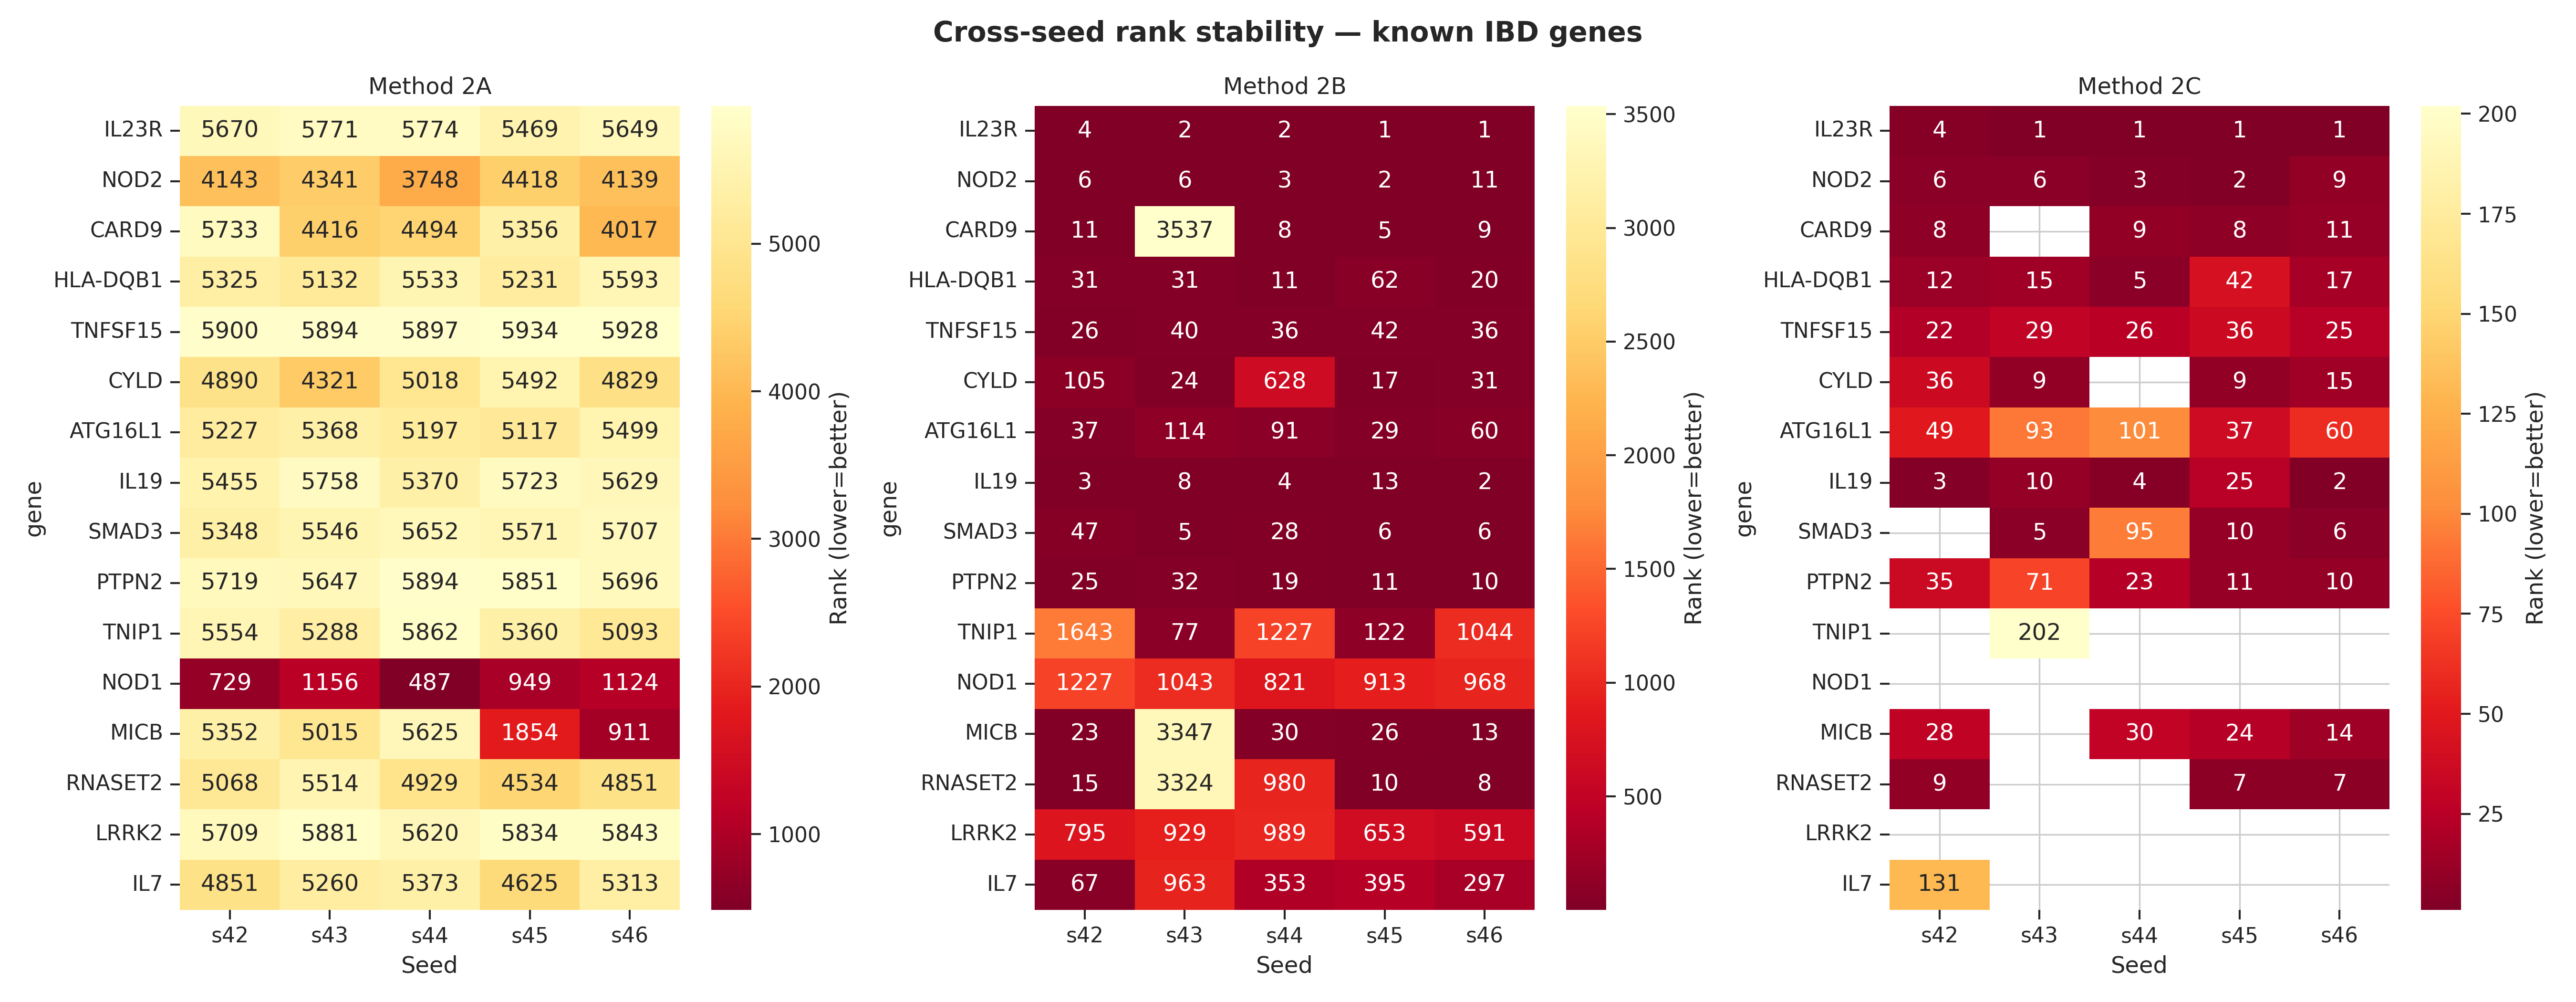
\includegraphics[height=0.78\textheight]{img/stability_heatmap.png}
        \caption{\small Cross-seed rank of known IBD genes under 2A / 2B / 2C (low = important).}
    \end{figure}
\end{frame}

\begin{frame}{Gene Importance Results: Reading the Heatmap}
    % [UPDATED 2026-06-18] left = explanation, right = ranks.
    % from results/multiseed_stability/stability_2A/2B/2C.csv (tanh, seeds 42-46).
    \small
    \begin{columns}[T]
        \begin{column}{0.55\textwidth}
            \metroset{block=fill}
            \begin{block}{Key finding}
                \footnotesize
                \begin{itemize}
                    \item \textbf{2A (weights)} ranks the known IBD genes \textbf{4{,}000--6{,}000+} (hub bias);
                          its top gene is the artifact \texttt{UBE2J2}.
                    \item \textbf{2B (SHAP)} \& \textbf{2C (perturbation)} recover them at ranks \textbf{1--40},
                          \emph{consistently across all 5 seeds}.
                \end{itemize}
            \end{block}
            \begin{block}{Take-away}
                \footnotesize
                Weight magnitude reflects \textbf{connectivity}, not predictive role; the data-driven
                methods (B, C) are what surface the real IBD biology --- and agree with each other.
            \end{block}
        \end{column}
        \begin{column}{0.45\textwidth}
            \centering
            \scriptsize
            \textbf{Top IBD genes --- mean rank (seeds 42--46)}\\[3pt]
            \renewcommand{\arraystretch}{1.2}
            \begin{tabular}{l c c}
                \toprule
                \textbf{Gene} & \textbf{2C rank} & \textbf{2B rank} \\
                \midrule
                IL23R    & \textbf{1.6} & \textbf{2.0} \\
                NOD2     & 5.2  & 5.6 \\
                IL19     & 8.8  & 6.0 \\
                HLA-DQB1 & 18.2 & 31.0 \\
                TNFSF15  & 27.6 & 36.0 \\
                PTPN2    & 30.0 & 19.4 \\
                \bottomrule
            \end{tabular}\\[4pt]
            \footnotesize ranks averaged across seeds 42--46 (lower = better).
        \end{column}
    \end{columns}
\end{frame}

% ----------------------------------------------------------------------------
% NEW [2026-06-18]: gene/interaction comparison vs van Hilten et al. Suppl. Sec 10
% (CPDB-pathway run = SAME architecture as ours). Overlaps verified against
% stability_2B/2C.csv and the suppl. interaction tables (Tables 3-5, Sec 13).
% ----------------------------------------------------------------------------
\begin{frame}{Comparison with SOTA: Genes \& Interactions}
    \small
    \begin{block}{Same architecture, same data}
        \footnotesize
        van Hilten et al.\ (Suppl.\ Sec~10) run a \textbf{CPDB-pathway} GenNet on the \emph{same} IIBDGC cohort,
        same hyperparameters (200 ep, L1 0.01, bs 64, lr $10^{-4}$) --- our exact setup.
        AUC matches: ours (ReLU) \textbf{0.726} $\approx$ their additive-encoding \textbf{0.722}.
    \end{block}
    \begin{columns}[T]
        \begin{column}{0.5\textwidth}
            \metroset{block=fill}
            \begin{block}{Genes recovered by both}
                \footnotesize
                Top of our SHAP / perturbation \emph{and} in their CPDB significant-gene list:
                \begin{itemize}
                    \item \textbf{IL23R, NOD2, SMAD3, HLA-DQB1}
                    \item HLA class-II cluster: HLA-DQA1, HLA-DRB1
                \end{itemize}
                Their non-coding hits (LINC*, \texttt{Y\_RNA}, pseudogenes) are absent from our pathway-pruned gene set.
            \end{block}
        \end{column}
        \begin{column}{0.5\textwidth}
            \metroset{block=fill}
            \begin{block}{Interactions agree}
                \footnotesize
                Their strongest pair: \textbf{NOD2 $\leftrightarrow$ IL23R}; \textbf{CARD9} an interaction hub
                (CARD9--GRB7, CARD9--LINC01845).
                \\[3pt]
                Our \textbf{DFIM} independently makes \textbf{CARD9} the interaction hub (top partner IL23R).
                In \emph{both} works CARD9 is weak in \emph{marginal} importance (our 2B rank 714) --- it shows up
                \textbf{only through interactions}.
            \end{block}
        \end{column}
    \end{columns}
    \vspace{0.05cm}
    \centering\scriptsize
    Reference: van Hilten et al., Supplementary Sec~10 (Interactions Between Genes, CPDB run) \& Tables~3--5.
\end{frame}

\begin{frame}{From GenNet to Individual-Specific Networks}
    % [UPDATED 2026-06-18] reflects what was actually built: gene selection -> two ISN engines.
    \small
	\textbf{Objective:} turn the trained network into one biological graph \emph{per patient}.

	\begin{block}{Step 1 --- Node selection (done)}
		\footnotesize
		Top-$N$ genes by the validated cross-seed SHAP rank (\texttt{stability\_2B}):
		IL23R, NOD2, IL19, SMAD3, PTPN2, JAK2, HLA-DQB1, \dots\ Cutoffs swept $50/100/150/200/250$.
	\end{block}

	\begin{block}{Step 2 --- ISN construction with LIONESS}
		\footnotesize
		For each patient we build a single-sample gene--gene network with \textbf{LIONESS}.
		\begin{itemize}
			\item \textbf{Node value:} per patient, one number per selected gene --- its
			      \textbf{GenNet gene-layer activation} (the value that gene's neuron outputs for that
			      patient). LIONESS treats this like a ``gene expression'' signal.
			\item \textbf{Output:} one $N\times N$ signed edge network per patient.
		\end{itemize}
	\end{block}
	\centering\footnotesize
	\textit{Activations are \textbf{tanh} (between $-1$ and $+1$, so they can be negative) $\rightarrow$ Phase~3--4 run on the tanh model, seed~42.}
\end{frame}

\begin{frame}{ISN Construction with LIONESS}
    % [KEEP] — matches project_context.md §3.3
	\small
	\textbf{Idea:} compare each patient's network to the population network. LIONESS does this with a
	\textbf{leave-one-out} estimate --- we do not hand-build the edges.

	\begin{block}{What LIONESS computes (per patient $k$)}
		\footnotesize
		For each patient, LIONESS estimates a single-sample network by leaving that patient out of the
		aggregate (population) network. Each edge measures how patient $k$ \textbf{deviates} from the
		population network $\rightarrow$ edges are \textbf{signed} ($+$/$-$).
	\end{block}

	\begin{columns}[T]
		\begin{column}{0.5\textwidth}
			\metroset{block=fill}
			\begin{block}{Input \& cutoff}
				\footnotesize
				\begin{itemize}
					\item Input = patient $\times$ gene \textbf{activation} matrix (Step~1 node values).
					\item \textbf{Cutoff $N$} = number of genes --- a tunable parameter, swept $50/100/150/200/250$.
					\item More genes $\rightarrow$ richer network but $N^2$ edges (more compute / disk).
				\end{itemize}
			\end{block}
		\end{column}
		\begin{column}{0.5\textwidth}
			\metroset{block=fill}
			\begin{block}{Output}
				\footnotesize
				\begin{itemize}
					\item One $N\times N$ gene--gene network \textbf{per test patient} (9{,}942).
					\item top250 $\rightarrow$ 62{,}500 edges/patient.
					\item Run on seed~42, all cutoffs.
				\end{itemize}
			\end{block}
		\end{column}
	\end{columns}
\end{frame}

\begin{frame}{ISN Results: LIONESS Single-Patient Networks}
    % [UPDATED 2026-06-18] image-only slide. Figure = results/lioness/top250_seed42/lioness_top_100.png
    % (LIONESS-generated top-100 strongest-edges plot), copied to img/isn_lioness_top250.png.
    \begin{figure}
        \centering
        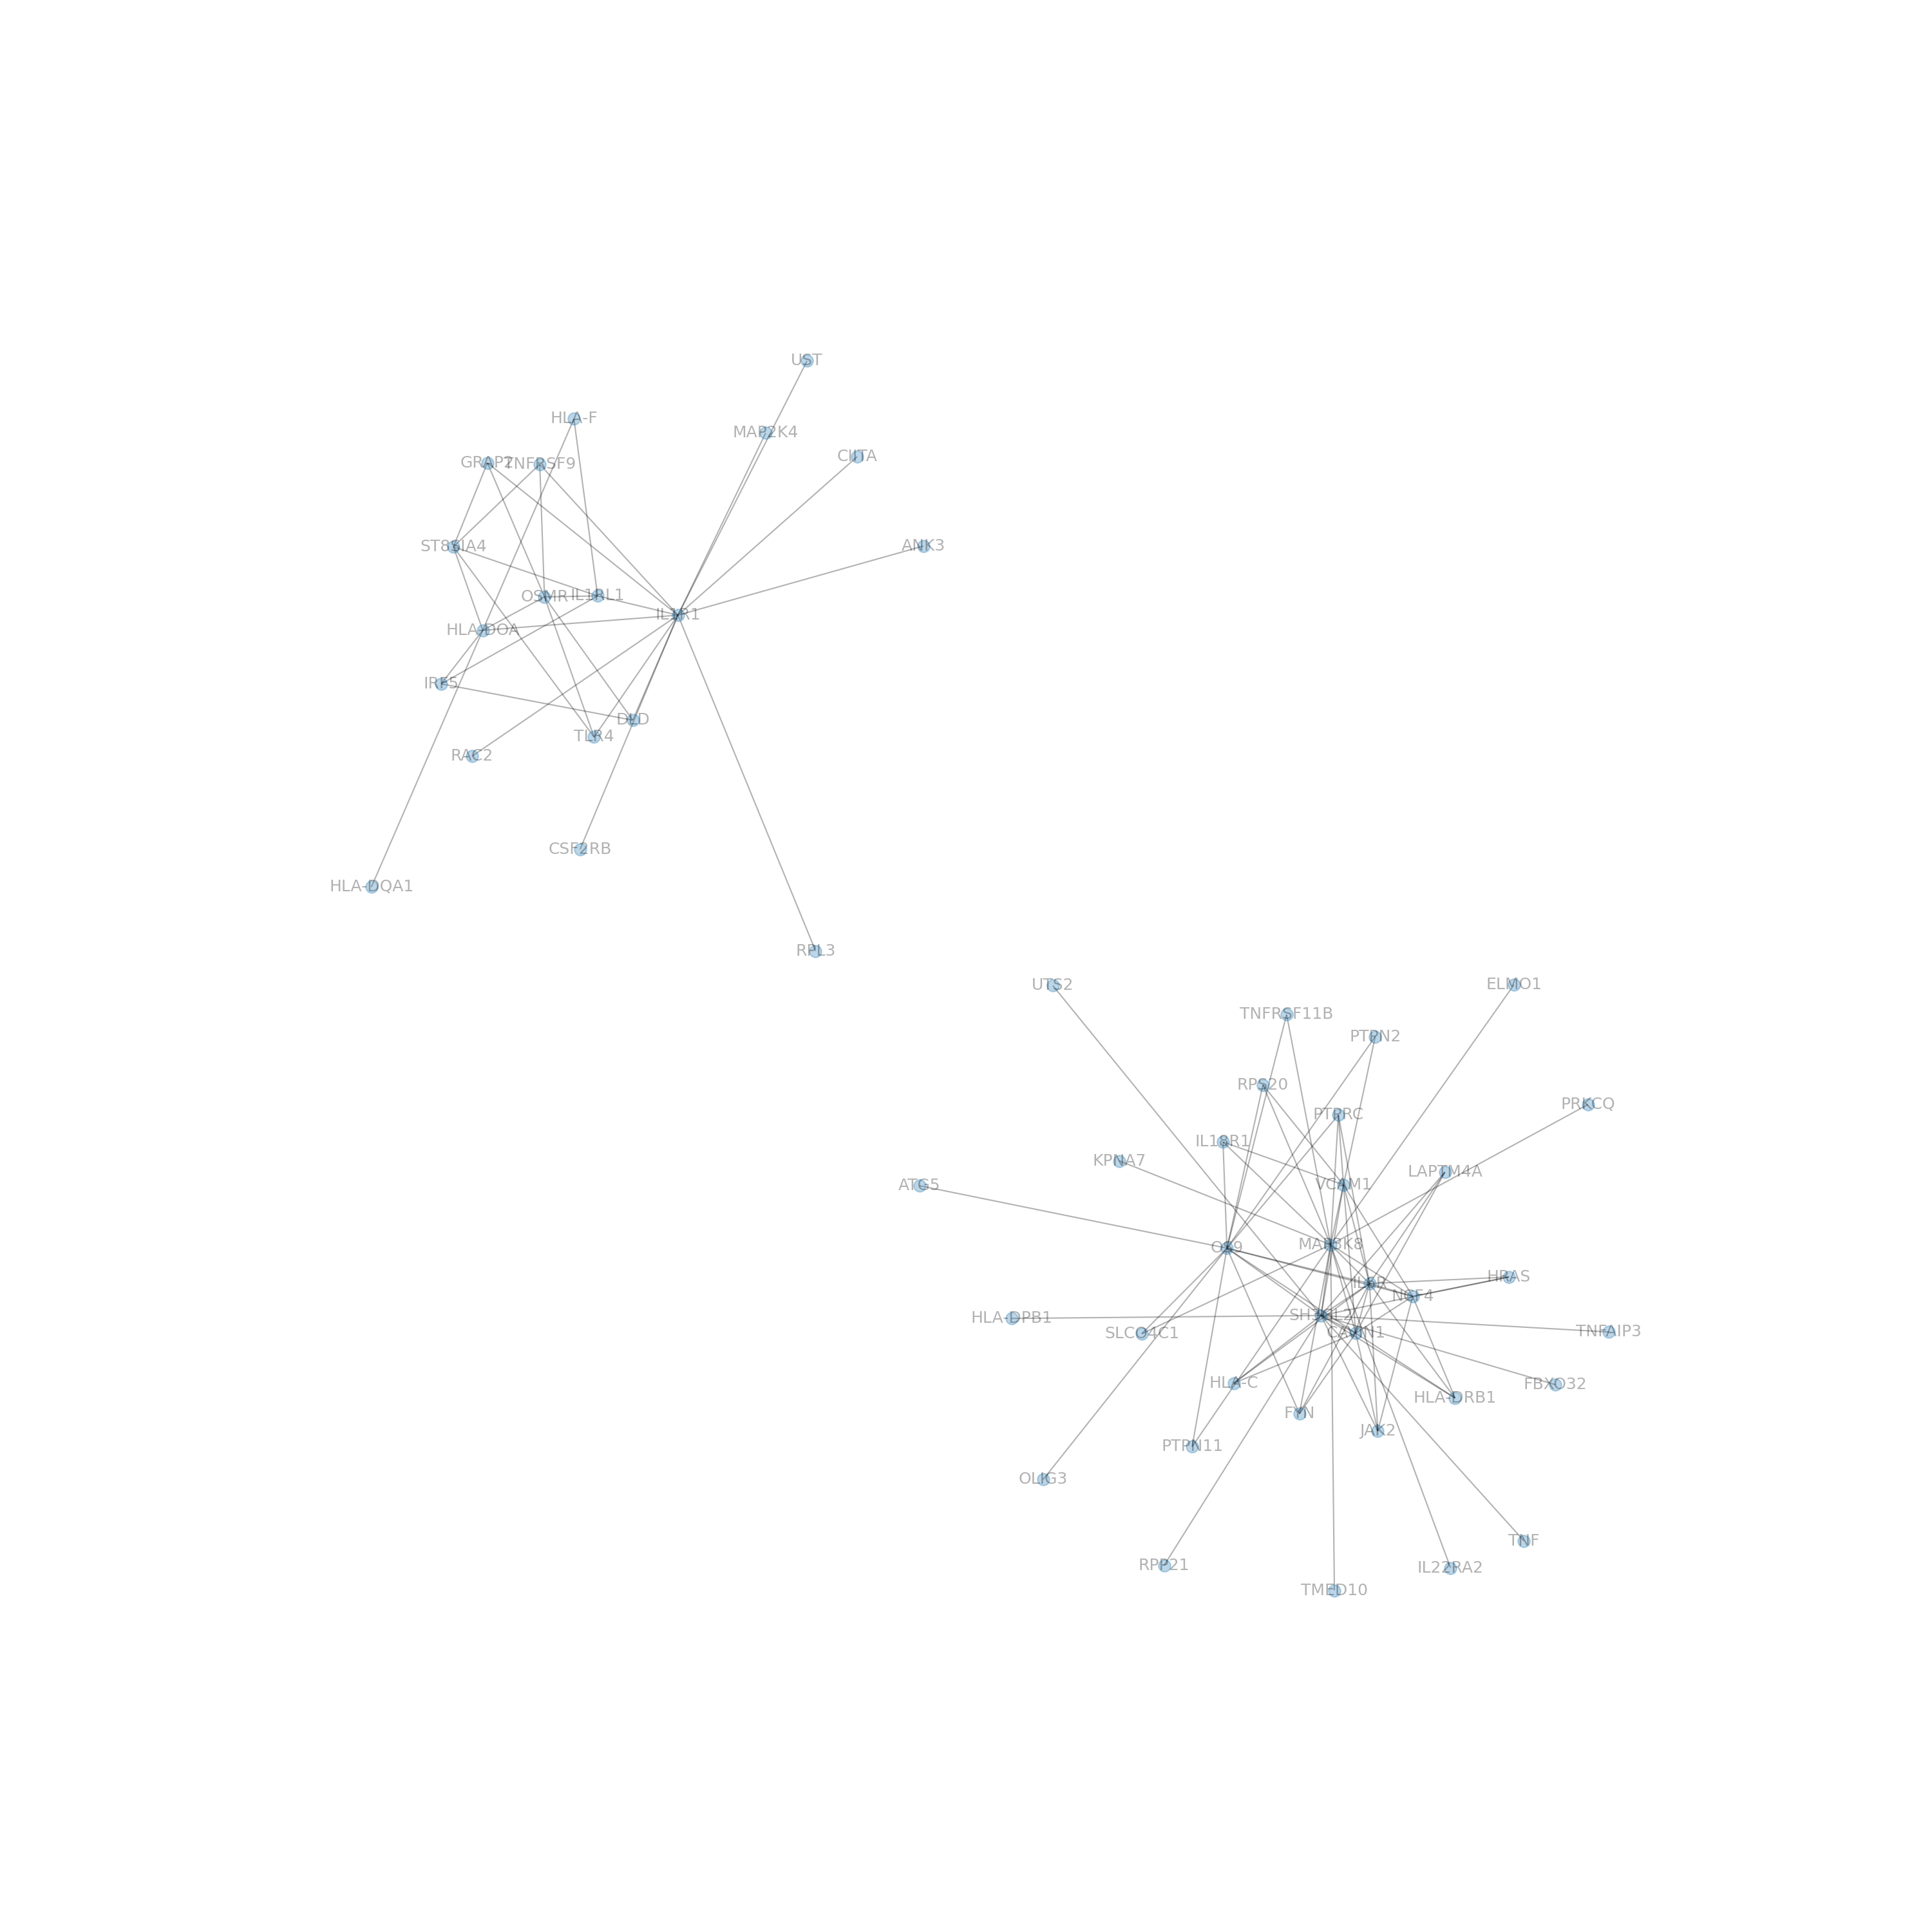
\includegraphics[height=0.78\textheight]{img/isn_lioness_top250.png}
        \caption{\small Top-100 strongest edges of a LIONESS ISN (top-250 gene set, seed~42).}
    \end{figure}
\end{frame}

\begin{frame}{ISN Results: What Was Produced}
    % [UPDATED 2026-06-18] from results/lioness/top{N}_seed42/ (seed 42, all 5 cutoffs).
    \small
    \begin{block}{What was produced}
        \footnotesize
        \begin{itemize}
            \item One signed $N\times N$ network for each of \textbf{9{,}942} test patients.
            \item Cutoffs $50\to250$ genes ($2{,}500\to62{,}500$ edges/patient).
            \item \textbf{Cleaned} (\texttt{clean\_lioness.py}): self-loops removed and bidirectional
                  duplicates collapsed --- each edge $i$--$j$ kept \textbf{once}.
        \end{itemize}
    \end{block}
    \footnotesize
    \textbf{Final output (input to HotZone):} one table per cutoff --- rows = unique gene--gene edges,
    columns = the \textbf{9{,}942 patients}; each cell = that edge's signed weight in that patient.
    \vspace{0.15cm}
    \centering\scriptsize \\
    \textbf{Method:} LIONESS leave-one-out; gene-layer (tanh) activations as the per-patient
    ``expression'' signal; seed~42, all cutoffs.
\end{frame}

% ============================================================================
\section{Phase 4 — HotZone analysis}
% ============================================================================

\begin{frame}{What is a HotZone?}
    % [TODO] definition from project_context.md §4
    \small
    \begin{block}{Definition}
        Many ISNs share the same node set, but edge weights vary across individuals.
        A \textbf{HotZone} is a subnetwork whose wiring \textbf{varies most strongly across individuals}.
    \end{block}
    \begin{itemize}
        \item Earlier work (Gaia) showed HotZones are more enriched for significant pathways than random subnetworks of the same size.
        \item \textbf{Detection (reproduces Gaia):} rank edges by cross-patient variance $\rightarrow$
              keep the high-variance graph $\rightarrow$ \textbf{Leiden communities}.
              Each community = one HotZone; their union = the \textbf{superhotzone}.
              Leiden is now \textbf{seeded} $\rightarrow$ reproducible zones.
    \end{itemize}
    \centering\footnotesize
    \textit{Three-step flow: (1) node selection from GenNet $\rightarrow$ (2) ISN + HotZone detection $\rightarrow$ (3) ``hotness'' scoring.}
\end{frame}

\begin{frame}{Scoring HotZone "Hotness"}
    % [UPDATED 2026-06-18] aligned with Kristel's note: full score D*E*S*C (+M for superhotzone);
    % this work implements simple D and E.
    \small
    Kristel's note --- hotness = composite of standardized components (per HotZone), plus a merge term
    for the superhotzone:
    \[ \text{hotness} = D^{*}\times E^{*}\times S\times C \qquad (\text{superhotzone: }\times\,M) \]
    \centering
    \renewcommand{\arraystretch}{1.2}
    \scriptsize
    \begin{tabular}{c l p{5.6cm}}
        \toprule
        \textbf{Sym} & \textbf{Component} & \textbf{What it measures} \\
        \midrule
        \textbf{D} & Differential wiring & how much internal wiring varies across individuals \\
        \textbf{E} & Enrichment & functional / pathway coherence \\
        S & Stability & reappearance under resampling \textit{(future)} \\
        C & Clustering & improves subtype discovery vs a baseline \textit{(future)} \\
        M & Merge coherence & superhotzone density / fragmentation / redundancy \textit{(future)} \\
        \bottomrule
    \end{tabular}
    \vspace{0.2cm}
    \begin{itemize}
        \footnotesize
        \item \textbf{In scope (per supervisor):} simple \textbf{D} and \textbf{E} $\rightarrow$ hotness $=D^{*}\times E^{*}$.
        \item Standardized vs \textbf{matched random subnetworks of the same size}: D vs the network null;
              E vs \emph{both} a matched-within-network null and a genome null.
        \item Report the \textbf{full component vector}, not only the scalar.
    \end{itemize}
\end{frame}

\begin{frame}{HotZone Results: Differential Wiring is the Signal}
    % [UPDATED 2026-06-18] results/hotzone_score/top250_seed42_Q98.0/ (seed 42, top250, Q98).
    \small
    Seed~42, top-250 gene set, threshold Q98 $\rightarrow$ \textbf{42-gene superhotzone}, 5 communities.
    \vspace{0.2cm}
    \centering
    \scriptsize
    \renewcommand{\arraystretch}{1.2}
    \begin{tabular}{l c | c c | c c}
        \toprule
        & & \multicolumn{2}{c|}{\textbf{D} (diff.\ wiring)} & \multicolumn{2}{c}{\textbf{E} (enrichment)} \\
        \textbf{Zone} & \textbf{genes} & $D^*$ & $p$ & $E^*$ matched & $E^*$ genome \\
        \midrule
        superhotzone & 42 & \textbf{6.15} & 0.001 & $-1.09$ (ns) & \textbf{+31.0} \\
        C0 & 14 & 4.60 & 0.001 & $-0.90$ (ns) & +7.1 \\
        C2 & 9  & 3.91 & 0.001 & $-0.82$ (ns) & +4.3 \\
        C3 & 6  & 3.34 & 0.002 & $+0.11$ (ns) & +5.9 \\
        C4 & 3  & 2.88 & 0.007 & $-0.42$ (ns) & +2.1 \\
        C1 & 10 & 2.32 & 0.007 & $-0.78$ (ns) & +10.2 \\
        \bottomrule
    \end{tabular}

    \vspace{0.3cm}
    \begin{itemize}
        \footnotesize
        \item \textbf{D is strong and significant everywhere} ($D^*$ up to 6.15, all $p\le0.007$) ---
              the real, distinctive signal. Zones collect canonical IBD/immune genes (IL23R, IFNG, JAK1, IRF4/8, TNFAIP3, HLA-DRA\dots).
        \item \textbf{E is baseline-dependent:} flat vs a matched within-network null (the node set is
              \emph{already} GenNet-selected IBD genes $\rightarrow$ ceiling), but large vs the genome null
              (reproduces Gaia's ``HotZones enriched vs random'').
    \end{itemize}
    \vspace{0.1cm}
    \centering\scriptsize
    \textbf{Method:} $D^*$ = z-score of within-zone edge variance vs 1000 matched-size random subnetworks;
    $E^*$ = standardized hypergeometric CPDB enrichment (matched + genome null); $p$ empirical.
\end{frame}

\begin{frame}{Downstream Proof-of-Concept}
    % [KEEP framing, project_context.md §2 Month 4: pick ONE]
	\textbf{Goal:} Apply ISNs/HotZones to a clinical question in IBD analysis (pick one).

	\vspace{0.3cm}
	\begin{columns}[T]
		\begin{column}{0.48\textwidth}
			\textbf{Option A: HotZone Prediction}
			\begin{itemize}
				\item Predict regional "HotZones" of inflammation from GenNet + ISN nodes.
				\item Reduce ISN construction to nodes that matter in a "HotZone sense".
			\end{itemize}
		\end{column}
		\begin{column}{0.48\textwidth}
			\textbf{Option B: Patient Clustering}
			\begin{itemize}
				\item ML-embedding of ISNs for unsupervised clustering.
				\item Identify \textbf{sub-phenotypes} of UC and CD.
			\end{itemize}
		\end{column}
	\end{columns}
	\vspace{0.4cm}
	\centering\footnotesize
	\textit{Pursued: \textbf{Option A}. HotZones detected from the LIONESS ISNs are scored for ``hotness''
	(D/E); differential wiring (D) cleanly separates them from matched random subnetworks.}
\end{frame}

% ============================================================================
\section{Conclusions}
% ============================================================================

\begin{frame}{Conclusions \& Next Steps}
    \begin{itemize}
        \item \textbf{Performance:} ReLU is the best GenNet configuration (val AUC \textbf{0.726}), competitive
              with the van Hilten et al.\ baseline.
        \item \textbf{Importance:} weight-based ranking is dominated by hub bias; \textbf{SHAP and
              perturbation are stable across seeds} and recover the right biology --- \textbf{IL23R} is the
              top, most-stable gene (mean rank 1.6--2.0), followed by NOD2 and IL19.
        \item \textbf{ISN:} per-patient LIONESS networks (top-250 genes, 9{,}942 patients) are coherent,
              with IL23R as a signed hub.
        \item \textbf{HotZone:} \textbf{differential wiring (D) is the real signal} ($D^*$ up to 6.15);
              enrichment (E) is baseline-dependent because the node set is already IBD-enriched.
    \end{itemize}
    \vspace{0.2cm}
    \begin{block}{Limitations \& outlook}
        \footnotesize
        Phase~3--4 currently run on the tanh model, seed~42 --- next: carry ReLU forward and extend
        LIONESS/HotZone to all 5 seeds (stability component S). Open methodological choice for the
        supervisor: the \textbf{E baseline} (matched vs genome).
    \end{block}
\end{frame}

% ============================================================================
\begin{frame}[t, allowframebreaks]{References}
	\begin{thebibliography}{99}
		\setbeamertemplate{bibliography item}{\insertbiblabel}
		\scriptsize

		\bibitem{Strober2007}
		Strober, W., Fuss, I., and Mannon, P.
		\newblock \emph{The fundamental basis of inflammatory bowel disease}.
		\newblock Journal of Clinical Investigation, 117(3):514-521, 2007.

		\bibitem{vanHilten2025}
		van Hilten, A., Melograna, F., Fan, B., et al.
		\newblock \emph{Detecting genetic interactions with visible neural networks}.
		\newblock Communications Biology, 8(1):874, 2025.

		\bibitem{Ellinghaus2016}
		Ellinghaus, D., Jostins, L., Spain, S. L., et al.
		\newblock \emph{Analysis of five chronic inflammatory diseases identifies 27 new associations}.
		\newblock Nature Genetics, 48(5):510-518, 2016.

		\bibitem{duroux2022interpretable}
		Duroux, D., Climente-González, H., Azencott, C. A., and Van Steen, K.
		\newblock \emph{Interpretable network-guided epistasis detection}.
		\newblock GigaScience, 11, 2022.

		\bibitem{liu2015association}
		Liu, J. Z., van Sommeren, S., Huang, H., et al.
		\newblock \emph{Association analyses identify 38 susceptibility loci for inflammatory bowel disease}.
		\newblock Nature Genetics, 47:979-986, 2015.

		\bibitem{hilten2021gennet}
		van Hilten, A., Kushner, S. A., Kayser, M., et al.
		\newblock \emph{GenNet framework: interpretable deep learning for predicting phenotypes from genetic data}.
		\newblock Communications Biology, 4, 2021.

	\end{thebibliography}
\end{frame}

\begin{frame}[standout]
    Thank you for your attention!
    \vspace{1.5cm}

    \normalsize{Kristian Kovacev - 885839} \\
\end{frame}

\end{document}

